\documentclass[10pt,aspectratio=169,serif]{beamer}

\usepackage[fontset=none, scheme=plain]{ctex}
\IfFontExistsTF{Songti SC}{%
	\setCJKmainfont{Songti SC}[AutoFakeSlant=0.2]%
	\setCJKsansfont{Songti SC}[AutoFakeSlant=0.2]%
}{%
	\setCJKmainfont{FandolSong-Regular}[Extension=.otf,BoldFont=FandolSong-Bold,AutoFakeSlant=0.2]%
	\setCJKsansfont{FandolSong-Regular}[Extension=.otf,BoldFont=FandolSong-Bold]%
}
\usepackage{amsmath,amssymb,graphicx,tikz,booktabs,multicol,calligra}
\usepackage{pgfplots}
\pgfplotsset{compat=1.18}
\usepackage{tcolorbox}
\tcbuselibrary{skins}
\usepackage{XyygU}
\usepackage{caption}
\captionsetup[figure]{name=图,labelsep=period}

\usetikzlibrary{arrows.meta,positioning,calc}

\setlength{\abovedisplayskip}{0pt plus 2pt minus 2pt}
\setlength{\belowdisplayskip}{0pt plus 2pt minus 2pt}

\title[5.7 三角函数的应用练习]{5.7 三角函数的应用（练习）}
\subtitle{简谐运动 \& 交变电流 \& 周期现象建模}
\author{}
\institute{}
\date{2026-10-16}

\begin{document}

\begin{frame}
  \titlepage
\end{frame}

% --- 1 ---
\begin{frame}[t]{第1题：简谐运动图象}
\textbf{1.} 某简谐运动的图象如图所示，试根据图象回答下列问题：
\begin{enumerate}
  \item 这个简谐运动的振幅、周期与频率各是多少？
  \item 写出这个简谐运动的函数解析式。
\end{enumerate}

\begin{center}
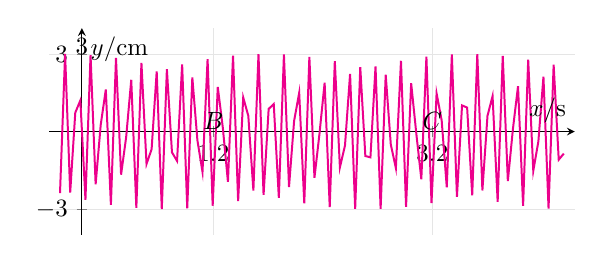
\begin{tikzpicture}[scale=0.9]
\begin{axis}[width=9cm,height=4.5cm,axis lines=middle,xlabel=$x$/s,ylabel=$y$/cm,
xmin=-0.3,xmax=4.5,ymin=-4,ymax=4,xtick={1.2,3.2},ytick={-3,3},
grid=major,grid style={gray!20}]
\addplot[thick,magenta,domain=-0.2:4.4,samples=100] {3*cos(deg(360*x/4.4))};
\node at (axis cs:0,3.3) {$3$};
\node at (axis cs:1.2,0.4) {$B$};
\node at (axis cs:3.2,0.4) {$C$};
\end{axis}
\end{tikzpicture}
\end{center}
\end{frame}

\begin{frame}[t]{第1题 解答}
\begin{tcolorbox}[colback=orange!10,colframe=orange,title=\textbf{解}]
(1) 由图读得：振幅 $A=3$ cm。
从 $x=0$（最高点）到最低点在 $x=2.2$（$B=1.2$ 与 $C=3.2$ 的中点），故半周期 $2.2$ s，周期 $T=4.4$ s。
频率 $f=\dfrac1T=\dfrac5{22}\approx 0.227$ Hz。

(2) 设 $y=A\cos(\omega t+\varphi)$，$A=3$，$\omega=\dfrac{2\pi}{T}=\dfrac{5\pi}{11}$。
$t=0$ 时 $y=3$ 为最高点，故 $\varphi=0$。
\[
\alert{y=3\cos\frac{5\pi}{11}t,\quad t\in[0,+\infty)}.
\]
\end{tcolorbox}
\end{frame}

% --- 2 ---
\begin{frame}[t]{第2题：沙漏单摆}
\textbf{2.} 一根绝对刚性且长度不变、质量可忽略不计的线，一端固定，另一端悬挂一个沙漏。沙漏在偏离平衡位置一定角度后在重力作用下做周期摆动。若线长为 $l$ cm，沙漏离开平衡位置的位移 $s$（单位：cm）与时间 $t$（单位：s）的函数关系为
\[
s=3\cos\!\left(\sqrt{\frac{g}{l}}\,t+\frac{\pi}{3}\right),\quad t\in[0,+\infty).
\]
\begin{enumerate}
  \item 当 $l=25$ 时，求该沙漏的最大偏角（精确到 $0.0001$ rad）；
  \item 已知 $g=9.8$ m/s$^2$，要使沙漏摆动的周期是 $1$ s，线的长度应当是多少（精确到 $0.1$ cm）？
\end{enumerate}
\end{frame}

\begin{frame}[t]{第2题 解答}
\begin{tcolorbox}[colback=orange!10,colframe=orange,title=\textbf{解}]
(1) 振幅 $3$ cm 即沙漏离开平衡位置的最大弧长位移为 $3$ cm。最大偏角 $\theta_{\max}$ 满足弧长 $s_{\max}=l\theta_{\max}$：
\[
\theta_{\max}=\frac{3}{25}=0.1200\ \text{rad}.
\]

(2) 周期 $T=\dfrac{2\pi}{\sqrt{g/l}}=2\pi\sqrt{\dfrac{l}{g}}$。令 $T=1$：
\[
l=\frac{g}{4\pi^2}=\frac{980}{4\pi^2}\approx 24.8\ \text{cm}.
\]
（注意 $g=9.8$ m/s$^2=980$ cm/s$^2$。）
\end{tcolorbox}
\end{frame}

% --- 3 ---
\begin{frame}[t]{第3题：发电机正弦电流}
\textbf{3.} 一台发电机产生的电流是正弦式电流，电压和时间之间的关系如图所示。由图象说出它的周期、频率和电压的最大值，并求出电压 $U$（单位：V）关于时间 $t$（单位：s）的函数解析式。

\begin{center}
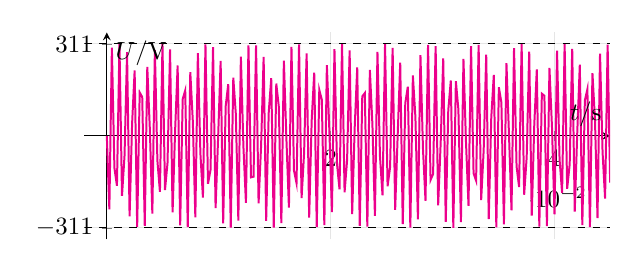
\begin{tikzpicture}[scale=0.9]
\begin{axis}[width=9cm,height=4.5cm,axis lines=middle,xlabel=$t$/s,ylabel=$U$/V,
xmin=-0.002,xmax=0.045,ymin=-350,ymax=350,xtick={0.02,0.04},ytick={-311,311},
grid=major,grid style={gray!20}]
\addplot[thick,magenta,domain=0:0.045,samples=200] {311*sin(deg(360*50*x))};
\draw[dashed] (axis cs:-0.002,311) -- (axis cs:0.045,311);
\draw[dashed] (axis cs:-0.002,-311) -- (axis cs:0.045,-311);
\end{axis}
\end{tikzpicture}
\end{center}
\end{frame}

\begin{frame}[t]{第3题 解答}
\begin{tcolorbox}[colback=orange!10,colframe=orange,title=\textbf{解}]
由图：电压最大值 $311$ V。$0.04$ s 内完成 $2$ 个周期，故周期 $T=0.02$ s，频率 $f=50$ Hz，$\omega=2\pi f=100\pi$。
$t=0$ 时 $U=0$ 且上升，故初相 $\varphi=0$：
\[
\alert{U=311\sin(100\pi t),\quad t\ge 0}.
\]
（有效值 $U_{\text{有}}=\dfrac{311}{\sqrt2}\approx 220$ V，即民用照明电压。）
\end{tcolorbox}
\end{frame}

% --- 4 ---
\begin{frame}[t]{第4题：绳波传播}
\textbf{4.} 下图为一向右传播的绳波在某一时刻绳子各点的位置图，经过 $\dfrac12$ 周期后，乙点的位置将移至何处？

\begin{center}
\begin{tikzpicture}[scale=1]
\draw[->] (-1,0) -- (8,0) node[right] {$x$};
\draw[->] (0,-5) -- (0,5) node[above] {$y$};
\draw[thick,magenta] plot[smooth] coordinates {(-1,-4)(0,0)(1,4)(2,0)(3,-4)(4,0)(5,4)(6,0)(7,-4)};
\draw[dashed] (-1,4) -- (7,4);
\draw[dashed] (-1,-4) -- (7,-4);
\node[above] at (1,4) {乙};
\node[above] at (5,4) {戊};
\node[below] at (0.5,0) {甲};
\node[below] at (2.5,0) {丙};
\node[below] at (3,-4) {丁};
\draw[->,thick] (5,4.8) -- (6.5,4.8);
\node[right] at (6.5,4.8) {$v$};
\end{tikzpicture}
\end{center}
\end{frame}

\begin{frame}[t]{第4题 解答}
\begin{tcolorbox}[colback=orange!10,colframe=orange,title=\textbf{解}]
乙点此时位于波峰 $y=4$。
经过半个周期，每个质点的振动状态相反：波峰处质点运动到波谷，即 $y=-4$。
（波向右传播，质点并不随波迁移，只在平衡位置附近上下振动。）

\alert{乙点将移到 $y=-4$ 的波谷位置（与图中丁点此时位置相同的高度）}。
\end{tcolorbox}
\end{frame}

% --- 5 ---
\begin{frame}[t]{第5题：人体生物节律（开放实践）}
\textbf{5.} 自出生之日起，人的体力、情绪、智力等心理、生理状况呈周期变化。体力节律 $23$ 天、情绪节律 $28$ 天、智力节律 $33$ 天。每个周期又分为高潮期、临界日和低潮期。生日前一天是起始位置（平衡位置）。请根据自己的出生日期，绘制自己的体力、情绪和智力曲线。
\end{frame}

\begin{frame}[t]{第5题 解答（方法指引）}
\begin{tcolorbox}[colback=orange!10,colframe=orange,title=\textbf{建模方法}]
设出生日（前一天）为 $t=0$，从平衡位置开始向上振动，则：
\[
y_{\text{体力}}=\sin\frac{2\pi t}{23},\qquad
y_{\text{情绪}}=\sin\frac{2\pi t}{28},\qquad
y_{\text{智力}}=\sin\frac{2\pi t}{33}.
\]
\begin{itemize}
  \item $y>0$ 为高潮期（体力充沛 / 情绪高昂 / 思维敏捷）；
  \item $y<0$ 为低潮期；
  \item $y=0$ 为临界日，注意平稳。
\end{itemize}
以出生日期为起点，按当前日期计算已出生天数 $t$，代入即可判断当日状态。
\end{tcolorbox}
\end{frame}

\begin{frame}[c]
  \begin{center}
    {\Huge\calligra Thanks!}
  \end{center}
\end{frame}

\end{document}
